\setlength\abovedisplayskip{2.5pt}

For relevant nuclear forensics predictions, both classification and regression
algorithms must be used.  For example, one may want to predict the reactor type
label given some measurement-based features of \gls{SNF} of an unknown source.
This would require a classification algorithm. Or perhaps the input fuel
composition is relevant to an investigation on weapons intent, so a regression
algorithm would be used to train a model based on some different set of
measured features. Since this work trains models to predict burnup of
\gls{SNF}, the algorithms are presented in a regression context.

\subsubsection{Linear Models}
\label{sec:linear}

One of the simplest and most utilized methods of prediction is a linear model
from a least-squares fit. Thus, it is the most natural place to begin a
demonstration of \gls{ML} algorithms. Since linear models must have all
linearly related parameters, there are many restrictions regarding the shape of
the model. However, this makes the resulting models stable to peturbations.
\cite{changingml}

\begin{figure}[!htb]
  \makebox[\textwidth][c]{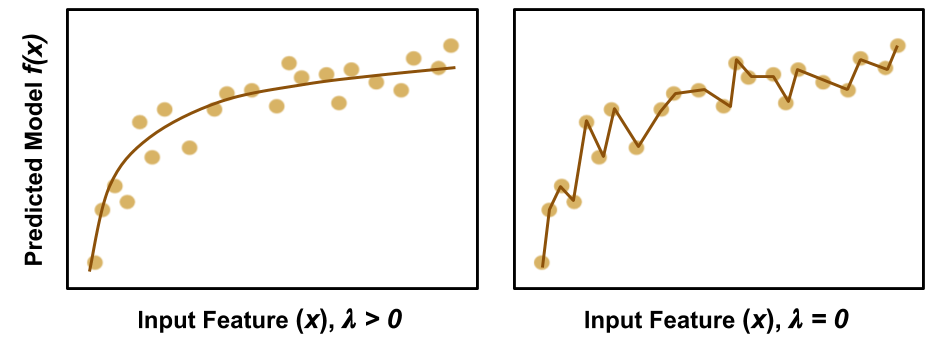
\includegraphics[width=1.1\textwidth]{./chapters/litrev/regularization.png}}
  \caption{Effect of Regularization on Prediction}
  \label{fig:reg}
\end{figure}

An example of a linear model is in Equation \ref{eq:linreg}. The vector of
input features of size $p$, $\boldsymbol{X}$, provides a model,
$F(\boldsymbol{X})$ by determining the unknown coefficients, or weights,
$\beta_{j}$'s. A loss function can be calculated by the difference in the
model-predicted value and $\boldsymbol{Y}$, the vector of actual labels.  The
algorithm calculates $\beta_{j}$ by minimizing the value of this loss function
over all the training data.  This is usually the least squares error from
minimizing the sum of squared errors, $\sum_{i=1}^{n} (y_i - f(x_i))^2$.  But
it could instead be the least absolute deviations from minimizing the sum of
absolute error differences, $\sum_{i=1}^{n} |y_i - f(x_i)|$. These are referred
to as the $L_2$ and $L_1$ norms, respectively.  
\begin{equation}
  F(\boldsymbol{X}) = \beta_{0} +  \sum_{j=1}^{p} x_{j} \beta_{j}
  \label{eq:linreg}
\end{equation}

The form of linear regression used here is called ridge regression. This
algorithm performs optimization using the $L_2$ norm, and also uses the form of
the $L_2$ norm for \textit{regularization}. Regularization, sometimes called
\textit{shrinkage}, is a term introduced into the \gls{ML} model to prevent
overfitting; it is used in many \gls{ML} algorithms. For ridge
regression, shrinkage further reduces the weights, $\beta_j$, on the input
features, $x_j$. The shrinkage term also includes a complexity parameter,
$\lambda$, which governs the strength to which regularization is performed
\cite{elements_stats}. Thus, the linear model given from ridge regression
is updated to Equation \ref{eq:ridgereg}.  Figure \ref{fig:reg} is a
visualization of how applying regularization smooths out a model.
\begin{equation}
  F(\boldsymbol{X}) = \beta_{0} +  \sum_{j=1}^{p} x_{j} \beta_{j} + \lambda \sum_{j=1}^{p} \beta_{j}^2
  \label{eq:ridgereg}
\end{equation}

\subsubsection{Nearest Neighbor Methods}
\label{sec:neighbor}

Nearest neighbor regression is a unique algorithm in that it is instance-based;
it does not actually generalize, but tracks the observations in the training
set.  The main metric for this algorithm is distance (or dissimilarity) between
the test sample and the closest training sample(s) in the vicinity.  During
prediction, the algorithm will calculate a value based on the instance that is
closest to the current test sample. Thus, there is not any learning, but
instead a direct comparison between an unknown sample and the space that the
training set populates. The predictions from nearest neighbors can be quite
accurate, but are highly unstable to peturbations \cite{elements_stats}.

\begin{figure}[!htb]
  \centering
  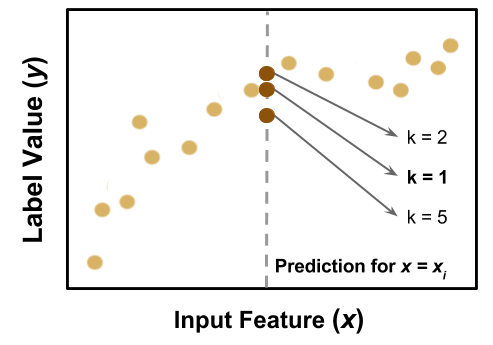
\includegraphics[width=0.8\linewidth]{./chapters/litrev/nn-fig.png}
  \caption{Schematic of \textit{k}-Nearest Neighbors Regression}
  \label{fig:nn}
\end{figure}

An extension of nearest neighbor is \textit{k}-nearest neighbor regression.
The closest \textit{k} neighbors are averaged for an estimate of the unknown
sample, as shown in Equation \ref{eq:knn}.  Figure \ref{fig:nn} provides a
pictoral explanation of how this is done for a prediction of a single feature.
For \textit{k}-neighbors, this algorithm predicts a value, $Y$, from the input
features, $\boldsymbol{X}$, in the neighborhood, $N_k (\boldsymbol{X})$
\cite{elements_stats}. 
\begin{equation}
  Y(\boldsymbol{X}) = \frac{1}{k} \sum_{x_i \in N_k(\boldsymbol{X})} y_i
  \label{eq:knn}
\end{equation}

There are two tuneable parameters in this algorithm: the distance metric and
the value of \textit{k}.  The population of the neighborhood, \textit{k},
affects the number of points being averaged together for a prediction.  The
metrics for distance differ, but in this study, the Euclidian distance was
used. In this initial work, $k = 1$ is used. This can perform very well, but
can also easily overfit the data and thus not generalize well. 

\subsubsection{Support Vector Machines}
\label{sec:svm}

\Acrfull{SVR} is an extension of the popular classification algorithm, \acrfull{SVM}.
This algorithm was chosen because of its ability to handle highly dimensional
data well, which in this study is a maximum of approximately 300 features. 

\begin{figure}[!htb]
  \centering
  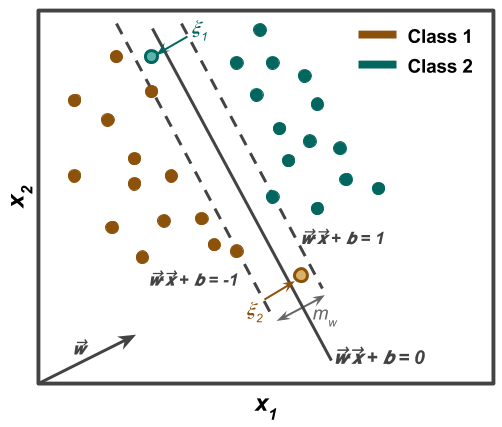
\includegraphics[width=0.8\linewidth]{./chapters/litrev/svm.png}
  \caption{Schematic of \acrshort{SVM} Classification}
  \label{fig:svm}
\end{figure}

As seen in Figure \ref{fig:svm}\footnote{This schematic is based on the
tutorial on SVMs by Dr.\@ Saed Sayad at
http://www.saedsayad.com/support\_vector\_machine.htm}, the \gls{SVM} algorithm
separates two classes by determining an optimal hyperplane between them.  The
algorithm evaluates the quality of the line that separates the two classes by
maximizing the margin width, $m_w = \frac{2}{\lVert w \rVert}$.  The hyperplane
is defined in Equation \ref{eq:plane}, where $\boldsymbol{w}$ is the vector
that is normal to the hyperplane.  
\begin{equation}
  \boldsymbol{w \cdot x} + b = 0
  \label{eq:plane}
\end{equation}

Figure \ref{fig:svm} also shows a case of soft margins.  Some problems are not
linearly separable, and thus a penalty term, $\xi_{i}$, is introduced to allow
for some misclassifications.  The algorithm then simultaneously minimizes the
misclassifications while maximizing the margin. The objective function of the
algorithm shows this as well (using quadratic programming) in Equation
\ref{eq:svm}. Here, $C$ is responsible for the margin width/misclassification
tradeoff, and the penalty term is included in the constraint. \cite{scikit,
elements_stats}
\begin{equation}
\begin{split}
  min\ & \frac{1}{2} \lVert w \rVert ^{2} + C \sum_{i} \xi_i \\
  subject\ to:\ \ & y_i (w x_i + b) > 1 - \xi_i
  \label{eq:svm}
\end{split}
\end{equation}

Figure \ref{fig:svr}\footnote{These schematics are based on a tutorial on SVR
by Dr.\@ Saed Sayad at
http://www.saedsayad.com/support\_vector\_machine\_reg.htm} demonstrates how
\gls{SVM} can be altered slightly from classification to nonlinear regression
with \gls{SVR}.  \Gls{SVR} has a similar objective function but instead
\textit{minimizes} the margin, as shown in Figure \ref{fig:svr-a}.  While the
objective function is the same as in Equation \ref{eq:svm}, the constraint is
now set to the opposite inequality sign, shown in Equation \ref{eq:svr} 
\begin{equation}
\begin{split}
  min\ & \frac{1}{2} \lVert w \rVert ^{2} + C \sum_{i} \xi_{i} \\
  subject\ to:\ \ & \lvert y_i - (w x_i + b) \rvert \leq \varepsilon + \xi_i
  \label{eq:svr}
\end{split}
\end{equation} 

Further, this can be extended to nonlinear analysis via what is called the
\textit{kernel trick}.  A nonlinear kernel function maps the data
into higher order feature space. The algorithm can then find a linear
separation in this space, as shown in Figure \ref{fig:svr-b}.

\begin{figure}[!hp]
  \centering
  \begin{subfigure}[h]{0.8\linewidth}
    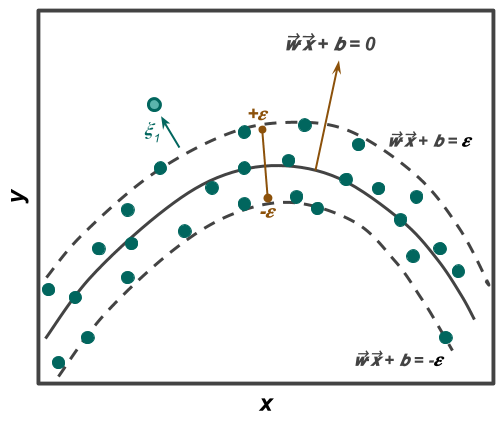
\includegraphics[width=\linewidth]{./chapters/litrev/svr-a.png}
    \caption{Demonstration of regression with \acrshort{SVR}}
    \label{fig:svr-a}
  \end{subfigure}
  \begin{subfigure}[h]{0.8\linewidth}
    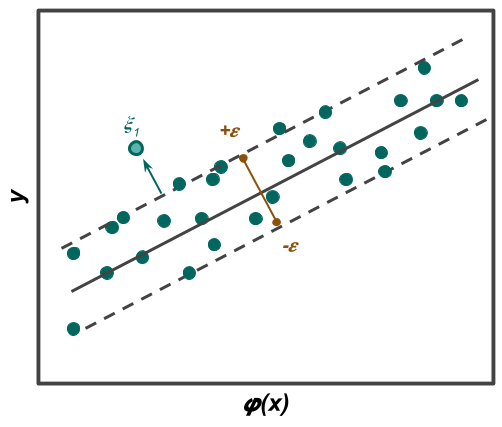
\includegraphics[width=\linewidth]{./chapters/litrev/svr-b.png}
    \caption{The kernel trick with \acrshort{SVR}}
    \label{fig:svr-b}
  \end{subfigure}
  \caption{Illustrations of \acrshort{SVR} and Nonlinear Analysis}
  \label{fig:svr}
\end{figure}

Chosen for its flexibility, the kernel in this study is the Gaussian radial
basis function, shown in Equation \ref{eq:svr-rbf}. This has two tuneable
parameters, $\gamma$ and $C$. The $\gamma$ controls the width of influence of
individual training instances, which strongly affects the fitting of the model.
Low values correspond to underfitting because the instances have too large of a
radius (low influence) and high values correspond to overfitting because the
instances have a small radius (high influence). 
\begin{equation}
\begin{split}
  min\ & \frac{1}{2} \lVert w \rVert ^{2} + C \sum_{i} \xi_{i} \\
  subject\ to:\ \ & \lvert y_i - (w \phi(x_i) + b) \rvert \leq \varepsilon + \xi_i \\
  where:\ & w = \sum_{i} \alpha_i y_i \phi(x_i) \\
  and:\ & K(x_i, x_j) = \phi(x_i) \phi(x_j) = e^{\gamma \lVert x_i - x_j \rVert ^{2}}
  \label{eq:svr-rbf}
\end{split}
\end{equation} 

The $C$ parameter also affects the fitting of the model by allowing more or
less support vectors, corresponding to more or less misclassification,
respectively. A lower $C$ smooths the surface of the model by allowing more
misclassifications, whereas a higher $C$ classifies more training examples by
allowing fewer misclassifications. Thus, too low or too high of a C can cause
under- or overfitting, respectively. 

Since there is a tradeoff of fitting strength provided by two parameters, it
is common to run the algorithm on a logarithmic grid from $10^{-3}$ to $10^3$
for each parameter. If plotted on a heatmap of accuracies given $\gamma$ and
$C$, there will be a diagonal of ideal combinations that emerges. The element
with the lowest value of each parameter is usually chosen. 

\subsubsection{Dimensionality Reduction Techniques}
\label{sec:dimreduc}

In addition to utilizing various algorithm parameters for regularization as
discussed above, dimensionality reduction can improve generalizability by
removing the noise of features that do not affect the regression task. This can
be thought of in the following way: shrinkage techniques reduce the weights of
noisy features, whereas dimensionality reduction removes them completely
\cite{elements_stats}.  Although one could use domain knowledge to manually
reduce the number of features in a data set (e.g., only including certain
nuclide subsets such as actinides), statistical feature reduction may also
prove helpful in this work.  The mathematical treatment of the methods
described below are in Ref.  \cite{elements_stats}.

%Another use for the following techniques is the visualization of one's data
%set, perhaps for data exploration or to show why certain predictions are
%difficult. 

\vspace{5mm} \noindent \textbf{Principal Components Analysis} \vspace{5mm}

\Gls{PCA} is considered the most common dimensionality reduction technique.
The \gls{PCA} algorithm learns a linear transformation of a data set
$\boldsymbol{X}$ with which to construct a transformation matrix according to a
user-chosen number of variables, i.e., components.  This matrix is part of the
singular value decomposition of the data matrix $\boldsymbol{X}$.  The
decomposition step is what provides the principal components, which are the
result of maximizing the variance in the original data while minimizing the
squared reconstruction error between the original data and the transformed
data. The mathematical assumptions are that the variables are all Gaussian and
uncorrelated.

Because the principal components are obtained purely statistically with no
model assumptions, they are usually uninterpretable. However, they can still
provide clues with which to obtain new information. In the case of this work,
this could provide insight into new forensics signatures.

\vspace{5mm} \noindent \textbf{Factor Analysis} \vspace{5mm}

Factor analysis is similar to \gls{PCA} in that it also calculates linear
combinations of the data set features using the above-mentioned decomposition
and the mathematical assumptions are the same.  It is different in that the
decomposition is rearranged so that it represents \textit{latent variables}
including random error disturbances rather than principal components.  Latent
variables are constructed by maximizing the correlation/shared variance among
the variables rather than the total variance.  However, different optimizations
can be chosen so that the solutions are parameter-dependent.  

Furthermore, the initial model assumptions, while enabling interpretable
results, also increase the dependence of the solutions on the algorithm inputs.
If \gls{PCA} does not perform well with the type of training data in this work,
it is possible that factor analysis will, since there are many nuclides in the
training data set that are in a decay chain together.

\vspace{5mm} \noindent \textbf{Independent Components Analysis} \vspace{5mm}

\Gls{ICA} has characteristics of both factor analysis and \gls{PCA}, but with
the goal of finding independent measurements from multiple `sources'.  It uses
the same form of decomposition as factor analysis but without the inclusion of
random error. The mathematical assumptions are a bit different: the variables
are statistically independent and non-Gaussian.  This allows the algorithm to
minimize higher-order statistics of the data set (\gls{PCA} and factor analysis
only minimize the first two orders).

Since the independent components are useful in signal processing of multiple
signals, this technique could prove useful for reprocessed nuclear materials
where multiple source streams converge. 

